%!TeX root=../sensetop.tex
\chapter[Chapter \thechapter]{}
\lettrine[lines=4,lraise=0.3]{A}{s} Elinor and Marianne were walking together the next morning the latter communicated a piece of news to her sister, which in spite of all that she knew before of Marianne’s imprudence and want of thought, surprised her by its extravagant testimony of both. Marianne told her, with the greatest delight, that Willoughby had given her a horse, one that he had bred himself on his estate in Somersetshire, and which was exactly calculated to carry a woman. Without considering that it was not in her mother’s plan to keep any horse, that if she were to alter her resolution in favour of this gift, she must buy another for the servant, and keep a servant to ride it, and after all, build a stable to receive them, she had accepted the present without hesitation, and told her sister of it in raptures.

»He intends to send his groom into Somersetshire immediately for it,« she added, »and when it arrives we will ride every day. You shall share its use with me. Imagine to yourself, my dear Elinor, the delight of a gallop on some of these downs.«

Most unwilling was she to awaken from such a dream of felicity to comprehend all the unhappy truths which attended the affair; and for some time she refused to submit to them. As to an additional servant, the expense would be a trifle; Mama she was sure would never object to it; and any horse would do for \textit{him}; he might always get one at the park; as to a stable, the merest shed would be sufficient. Elinor then ventured to doubt the propriety of her receiving such a present from a man so little, or at least so lately known to her. This was too much.

»You are mistaken, Elinor,« said she warmly, »in supposing I know very little of Willoughby. I have not known him long indeed, but I am much better acquainted with him, than I am with any other creature in the world, except yourself and mama. It is not time or opportunity that is to determine intimacy;—it is disposition alone. Seven years would be insufficient to make some people acquainted with each other, and seven days are more than enough for others. I should hold myself guilty of greater impropriety in accepting a horse from my brother, than from Willoughby. Of John I know very little, though we have lived together for years; but of Willoughby my judgment has long been formed.«

Elinor thought it wisest to touch that point no more. She knew her sister’s temper. Opposition on so tender a subject would only attach her the more to her own opinion. But by an appeal to her affection for her mother, by representing the inconveniences which that indulgent mother must draw on herself, if (as would probably be the case) she consented to this increase of establishment, Marianne was shortly subdued; and she promised not to tempt her mother to such imprudent kindness by mentioning the offer, and to tell Willoughby when she saw him next, that it must be declined.

She was faithful to her word; and when Willoughby called at the cottage, the same day, Elinor heard her express her disappointment to him in a low voice, on being obliged to forego the acceptance of his present. The reasons for this alteration were at the same time related, and they were such as to make further entreaty on his side impossible. His concern however was very apparent; and after expressing it with earnestness, he added, in the same low voice,—»But, Marianne, the horse is still yours, though you cannot use it now. I shall keep it only till you can claim it. When you leave Barton to form your own establishment in a more lasting home, Queen Mab shall receive you.«

This was all overheard by Miss Dashwood; and in the whole of the sentence, in his manner of pronouncing it, and in his addressing her sister by her Christian name alone, she instantly saw an intimacy so decided, a meaning so direct, as marked a perfect agreement between them. From that moment she doubted not of their being engaged to each other; and the belief of it created no other surprise than that she, or any of their friends, should be left by tempers so frank, to discover it by accident.

Margaret related something to her the next day, which placed this matter in a still clearer light. Willoughby had spent the preceding evening with them, and Margaret, by being left some time in the parlour with only him and Marianne, had had opportunity for observations, which, with a most important face, she communicated to her eldest sister, when they were next by themselves.

»Oh, Elinor!« she cried, »I have such a secret to tell you about Marianne. I am sure she will be married to Mr Willoughby very soon.«

»You have said so,« replied Elinor, »almost every day since they first met on High-church Down; and they had not known each other a week, I believe, before you were certain that Marianne wore his picture round her neck; but it turned out to be only the miniature of our great uncle.«

»But indeed this is quite another thing. I am sure they will be married very soon, for he has got a lock of her hair.«

»Take care, Margaret. It may be only the hair of some great uncle of \textit{his}.«

»But, indeed, Elinor, it is Marianne’s. I am almost sure it is, for I saw him cut it off. Last night after tea, when you and mama went out of the room, they were whispering and talking together as fast as could be, and he seemed to be begging something of her, and presently he took up her scissors and cut off a long lock of her hair, for it was all tumbled down her back; and he kissed it, and folded it up in a piece of white paper; and put it into his pocket-book.«

\begin{figure}[tbph]
\centering
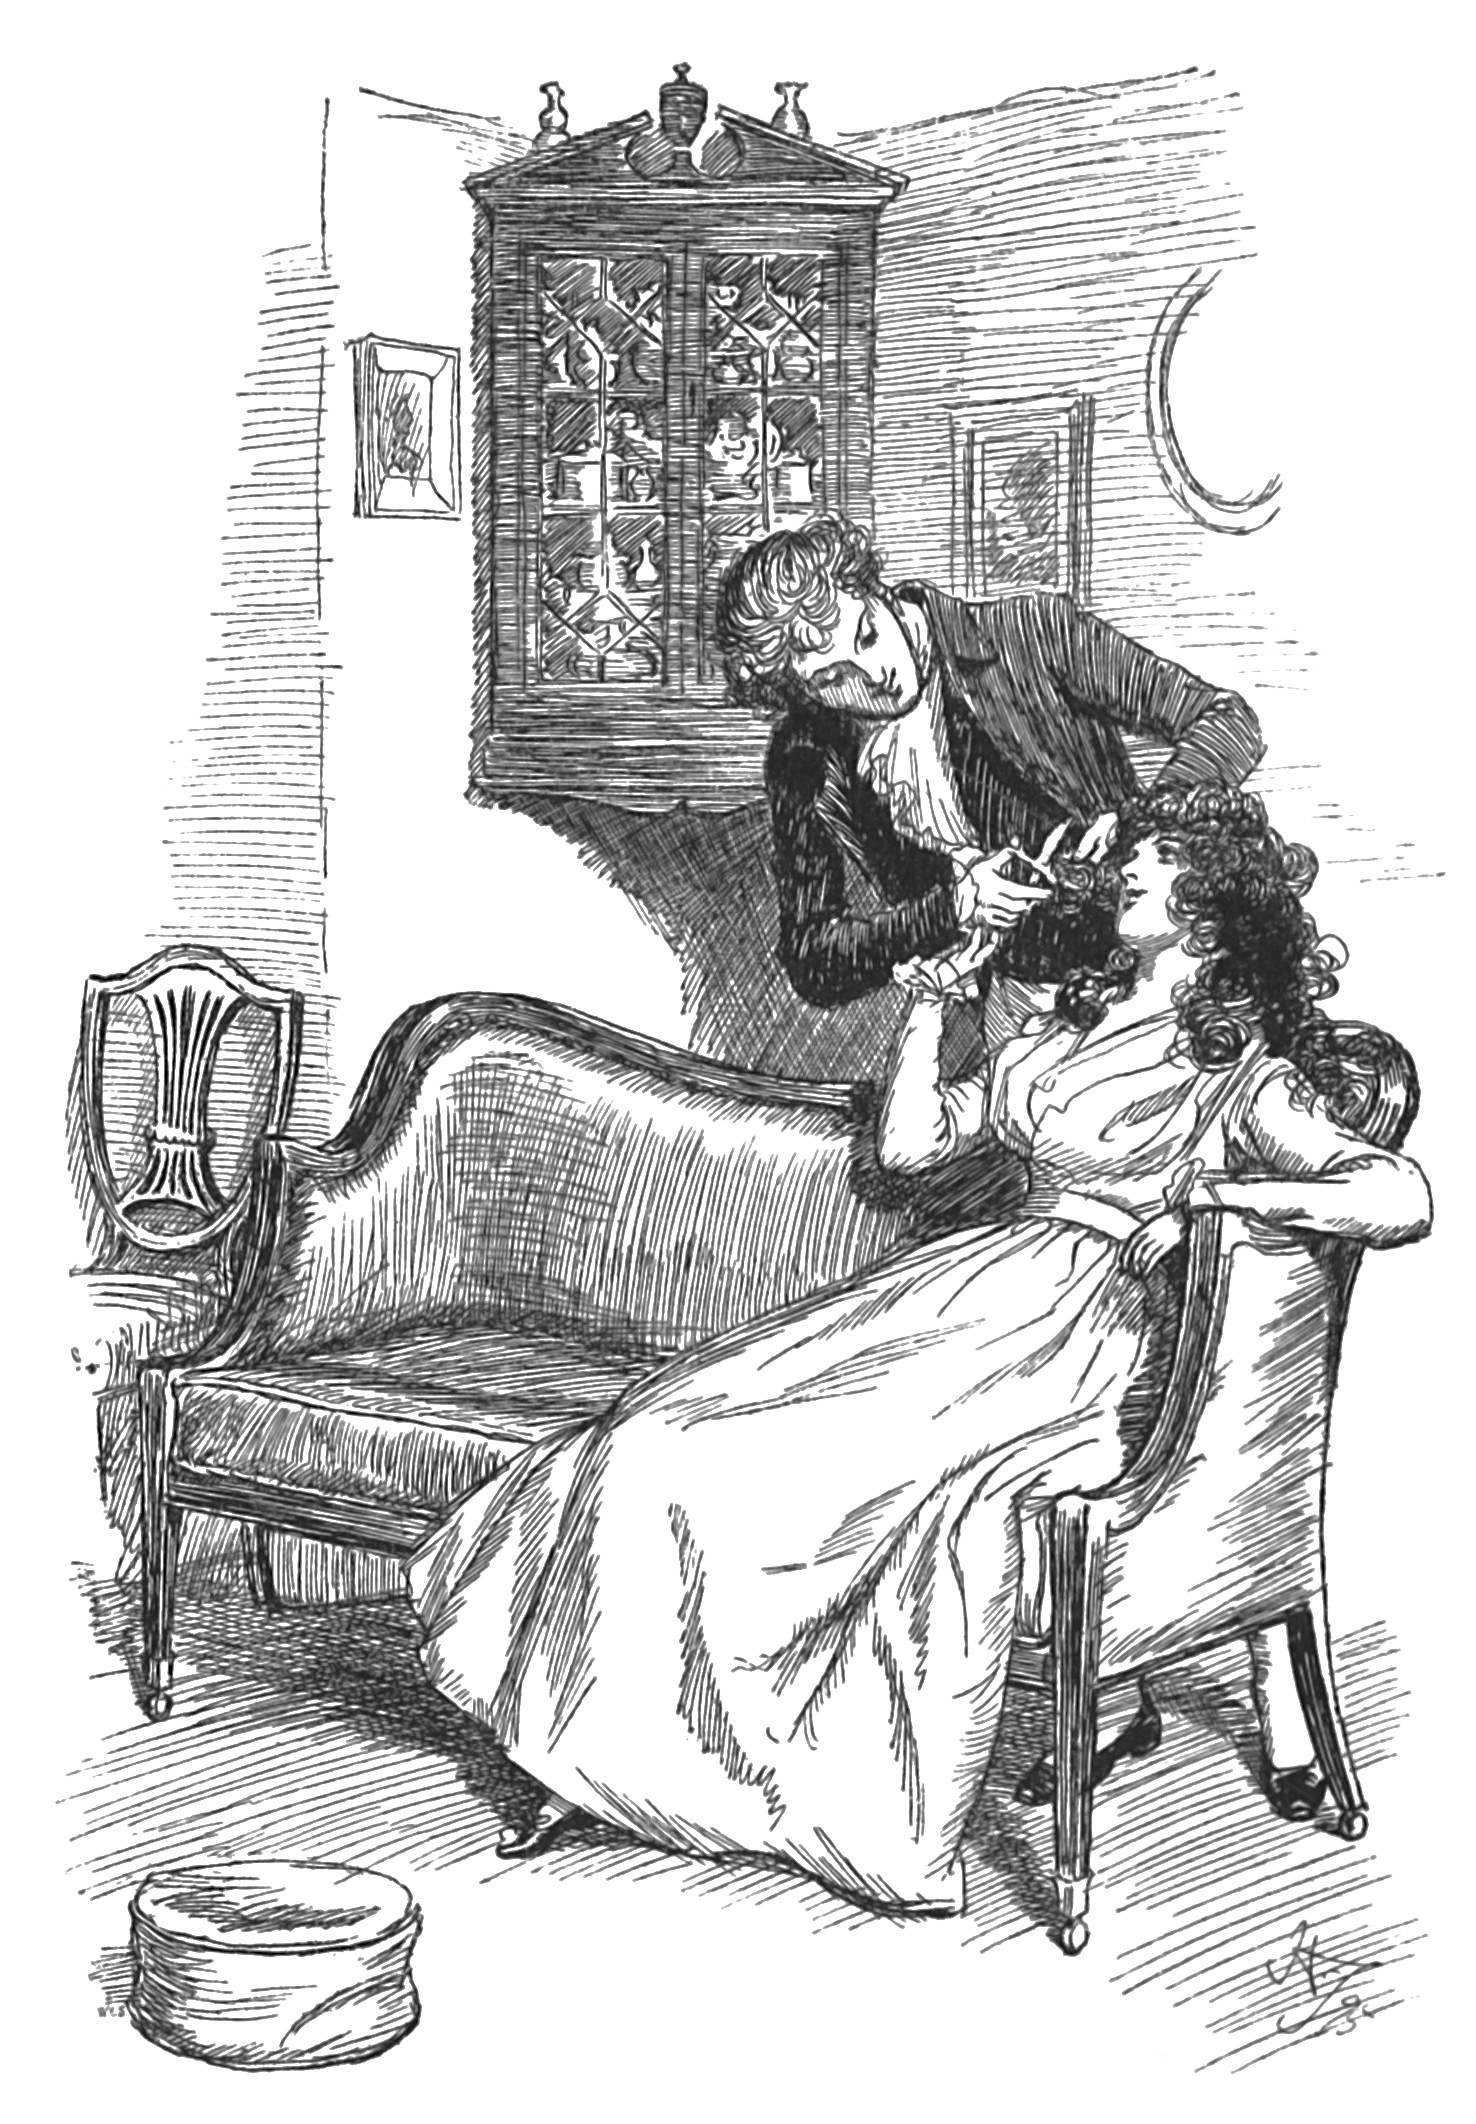
\includegraphics[width=\linewidth]{12lock}
\caption{He cut off a long lock of her hair}
\end{figure}

For such particulars, stated on such authority, Elinor could not withhold her credit; nor was she disposed to it, for the circumstance was in perfect unison with what she had heard and seen herself.

Margaret’s sagacity was not always displayed in a way so satisfactory to her sister. When Mrs Jennings attacked her one evening at the park, to give the name of the young man who was Elinor’s particular favourite, which had been long a matter of great curiosity to her, Margaret answered by looking at her sister, and saying, »I must not tell, may I, Elinor?«

This of course made every body laugh; and Elinor tried to laugh too. But the effort was painful. She was convinced that Margaret had fixed on a person whose name she could not bear with composure to become a standing joke with Mrs Jennings.

Marianne felt for her most sincerely; but she did more harm than good to the cause, by turning very red and saying in an angry manner to Margaret,

»Remember that whatever your conjectures may be, you have no right to repeat them.«

»I never had any conjectures about it,« replied Margaret; »it was you who told me of it yourself.«

This increased the mirth of the company, and Margaret was eagerly pressed to say something more.

»Oh! pray, Miss Margaret, let us know all about it,« said Mrs Jennings. »What is the gentleman’s name?«

»I must not tell, ma’am. But I know very well what it is; and I know where he is too.«

»Yes, yes, we can guess where he is; at his own house at Norland to be sure. He is the curate of the parish I dare say.«

»No, \textit{that} he is not. He is of no profession at all.«

»Margaret,« said Marianne with great warmth, »you know that all this is an invention of your own, and that there is no such person in existence.«

»Well, then, he is lately dead, Marianne, for I am sure there was such a man once, and his name begins with an F.«

Most grateful did Elinor feel to Lady Middleton for observing, at this moment, »that it rained very hard,« though she believed the interruption to proceed less from any attention to her, than from her ladyship’s great dislike of all such inelegant subjects of raillery as delighted her husband and mother. The idea however started by her, was immediately pursued by Colonel Brandon, who was on every occasion mindful of the feelings of others; and much was said on the subject of rain by both of them. Willoughby opened the piano-forte, and asked Marianne to sit down to it; and thus amidst the various endeavours of different people to quit the topic, it fell to the ground. But not so easily did Elinor recover from the alarm into which it had thrown her.

A party was formed this evening for going on the following day to see a very fine place about twelve miles from Barton, belonging to a brother-in-law of Colonel Brandon, without whose interest it could not be seen, as the proprietor, who was then abroad, had left strict orders on that head. The grounds were declared to be highly beautiful, and Sir John, who was particularly warm in their praise, might be allowed to be a tolerable judge, for he had formed parties to visit them, at least, twice every summer for the last ten years. They contained a noble piece of water; a sail on which was to form a great part of the morning’s amusement; cold provisions were to be taken, open carriages only to be employed, and every thing conducted in the usual style of a complete party of pleasure.

To some few of the company it appeared rather a bold undertaking, considering the time of year, and that it had rained every day for the last fortnight;—and Mrs Dashwood, who had already a cold, was persuaded by Elinor to stay at home.

\makeatletter
\@ifclasswith{scrbook}{a5paper}
{%
	\enlargethispage{\baselineskip}
}{%

}
\makeatother